% ─── Slide: ADC — pipeline + histograms ──────────────────────────────────────
\begin{frame}{ADC: Reading the Analog Accumulation}

  \vspace{-0.6em}
  \hfill\resizebox{0.6\linewidth}{!}{%
  \begin{tikzpicture}[
      every node/.style={font=\scriptsize},
      dq/.style={draw=mybluedark, rounded corners=2pt, fill=myblue!22,
                 minimum width=1.6cm, minimum height=0.68cm, align=center},
      tile/.style={draw=mybluedark, rounded corners=2pt, fill=mybluedark!15,
                   text=mybluedark, minimum width=2.0cm, minimum height=0.88cm,
                   align=center},
      adc/.style={draw=myorange, line width=1.5pt, rounded corners=2pt,
                  fill=myorange!35, minimum width=1.3cm, minimum height=0.68cm,
                  align=center},
      outbox/.style={draw, rounded corners=2pt, fill=mygreen!20,
                  minimum width=0.9cm, minimum height=0.68cm, align=center},
      arr/.style={-{Latex[length=1.3mm]}, thick},
      histbox/.style={draw=mygray!55, thin, rounded corners=2pt,
                      fill=white, inner sep=1pt},
      link/.style={dashed, mygray!60, line width=0.4pt}
    ]

    % ─── Pipeline ─────────────────────────────────────────────────────────
    \node[font=\Large] (wdots) at (3.0,  0.8) {$\cdots$};
    \node (wb)                  at (3.6,  0.8) {$\hat w$};

    \node[font=\Large] (xdots) at (3.0, -0.8) {$\cdots$};
    \node (xb)                  at (3.6, -0.8) {$\hat x$};

    \node[tile] (T) at (5.8, 0) {Optical MVM\\$y{=}\langle\hat w,\hat x\rangle$};
    \draw[arr] (wb) -- (T.north west);
    \draw[arr] (xb) -- (T.south west);

    \node (y)  at (7.6, 0) {$y$};
    \draw[arr] (T) -- (y);

    \node[adc] (A) at (8.9, 0) {ADC\\$\lfloor y/\delta\rfloor$};
    \draw[arr] (y)--(A);

    \node (yb) at (10.3, 0) {$\hat y$};
    \draw[arr] (A)--(yb);

    % ─── Orange zone: only ADC pipeline (NOT histograms) ──────────────────
    \begin{pgfonlayer}{background}
      \node[inner sep=9pt, draw=myorange, line width=1.5pt,
            rounded corners=7pt, fill=myorange!5,
            fit=(y)(A)(yb)] (Z2) {};
    \end{pgfonlayer}
    % ─── Histograms (outside the red frame) ───────────────────────────────
    \node[histbox] (hy)  at (7.6,  3.0) {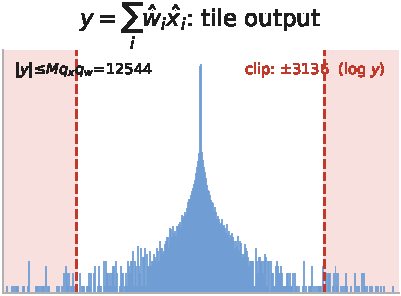
\includegraphics[width=2.6cm]{figs/dist_y.pdf}};
    \node[histbox] (hyb) at (10.3, -2.0) {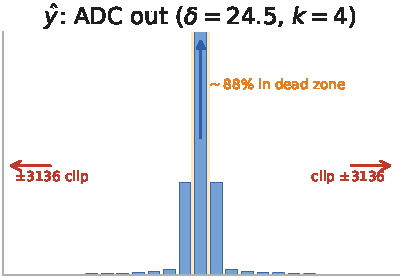
\includegraphics[width=2.6cm]{figs/dist_y_hat.pdf}};
    \draw[link] (hy.south)  -- (Z2.north -| hy);
    \draw[link] (hyb.north) -- (Z2.south -| hyb);

  \end{tikzpicture}}\hspace*{0pt}

  \vspace{-3.5cm}
  \begin{flushleft}
    \normalsize
    \onslide<1->{\textbf{\color{myorange}$\delta$ fix}}\par
    \smallskip
    \onslide<2->{\textbf{\color{myred}Can not do QAT on LLM}}\par
    \smallskip
    \onslide<3->{\textbf{\color{mybluedark}Can PTQ be done?}}
  \end{flushleft}

  \note{Зум в оранжевый прямоугольник. ADC читает аналоговый результат с фиксированным шагом delta — задан при производстве чипа. Если y попадает в мёртвую зону — обнуляется.}

\end{frame}
